\documentclass[a4paper, 14pt]{extarticle}

\usepackage{../generalPreamble}
\usepackage{../reportFormat}
\setcounter{MaxMatrixCols}{20}

\newcommand\sbullet[1][.5]{\mathbin{\vcenter{\hbox{\scalebox{#1}{$\bullet$}}}}}

\begin{document}

\begin{titlepage}
    \centering
    {\bfseries
        \uppercase{
            Минобрнауки России \\
            Санкт-Петербургский государственный \\
            Электротехнический университет \\
            \enquote{ЛЭТИ} им. В.И.Ульянова (Ленина)\\
        }
        Кафедра ИБ

        \vspace{\fill}
        \uppercase{Лабораторная работа №5} \\
        по дисциплине \enquote{Криптография и защита информации} \\
        Тема: Изучение шифра AES
    }

    \vspace{\fill}
    \begin{tabularx}{0.8\textwidth}{l X c r}
        Студент гр. 6304 & & \underline{\hspace{3cm}} & Корытов П.В.\\
        Преподаватель & & \underline{\hspace{3cm}} & Племянников А.К.
    \end{tabularx}

    \vspace{1cm}
    Санкт-Петербург \\
    \the\year{}
\end{titlepage}

\newpage

\section{Цель работы}
Цель работы: исследовать шифр AES, финалистов конкурса AES, атаку предсказанием дополнения и получить практические навыки работы с шифрами и атакой, в том числе и в программном продукте Cryptool 1 и 2.

\section{Основные теоретические положения}
Используется не сеть Фейстеля, а Square-like структура.
\begin{figure}[h]
    \centering
    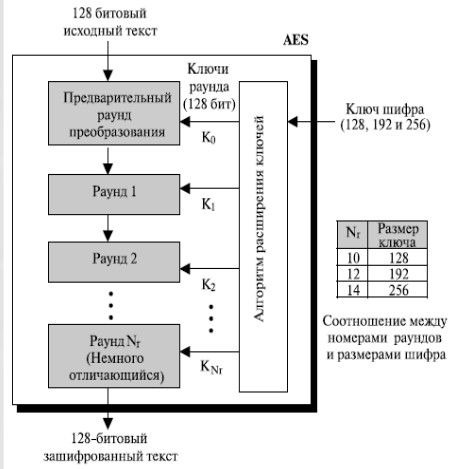
\includegraphics[width=0.7\textwidth]{img/S001.jpg}
    \caption{Структура шифра}%
\end{figure}

\subsection{Обще описание шифра}
\begin{itemize}
    \item Операции проводятся над элементами поля Галуа $GF(2^8)$.\\
    Т.е. байту соответстует многочлен $b_7 x^7 + b_6 x^6 + b_5 x^5 + b_4 x^4 + b_3 x^3 + b_2 x^2 + b_1 x + b_0$
    \item Операция умножения выполняется по модулю неприводимого многочлена $ x^8 + x^4 + x^3 + x + 1 $\\
\end{itemize}
Размер блока --- 16 байт, размер ключа --- 16, 24 или 32 байт. Размер матрицы состояний --- $4\times4$ блока

\begin{figure}[h]
    \centering
    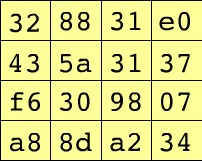
\includegraphics[width=0.3\textwidth]{img/S002.jpg}
    \caption{Матрица состояний}
\end{figure}

\begin{figure}[h]
    \centering
    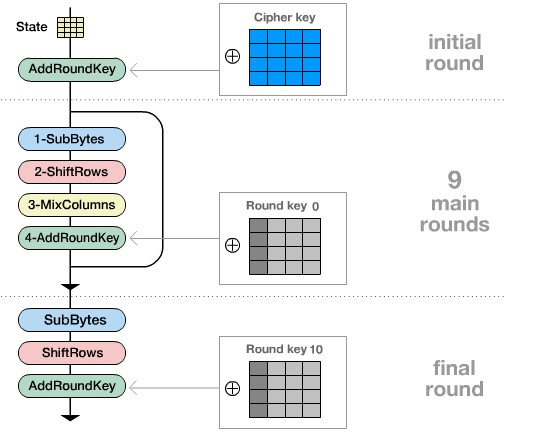
\includegraphics[width=0.8\textwidth]{img/S003.jpg}
    \caption{Операции шифра AES-192}
\end{figure}

\FloatBarrier{}
\subsection{Операции шифра}
Нижеописанные операции выполняются для всех раундов, кроме MixColumns --- она не выполняется для последнего раунда.
\subsubsection{SubBytes}
Производится нелинейная замена байтов с использованием таблицами Rijndael S-box.

\begin{figure}[h]
    \centering
    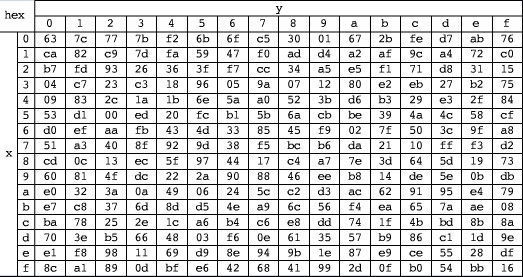
\includegraphics[width=0.9\textwidth]{img/S004.jpg}
    \caption{S-box}
\end{figure}
Первая цифра в шестнадцатеричной записи ключа --- строка, вторая --- столбец. Например, ``19'' становится ``d4''.

\FloatBarrier{}
\subsubsection{ShiftRows}
Первая строка сдвигается на 1 байт, вторая --- на 2, третья --- на 3.
\begin{figure}[h]
    \centering
    \begin{subfigure}[b]{0.3\textwidth}
    	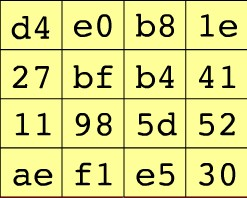
\includegraphics[width=\textwidth]{img/S006.jpg}
    	\caption{Вход ShiftRows}
    \end{subfigure}%
    \hspace{1cm}
    \begin{subfigure}[b]{0.3\textwidth}
    	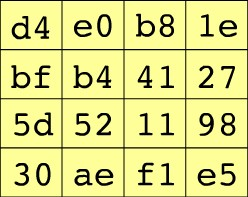
\includegraphics[width=\textwidth]{img/S007.jpg}
    	\caption{Выход ShiftRows}
    \end{subfigure}
\end{figure}

\subsubsection{MixColumns}
Каждый столбец представляется как полином третьем степени. Он умножается в $GF(2^8)$ по модулю $x^4 + 1$ на многочлен $3x^3 + x^2 + x + 2$.
\begin{figure}[h]
    \centering
    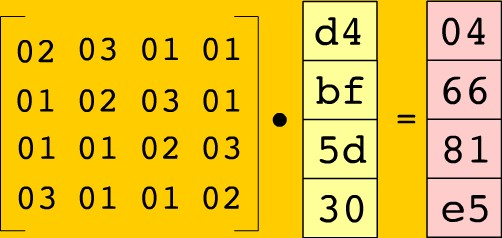
\includegraphics[width=0.4\textwidth]{img/S008.jpg}
    \caption{MixColumns}
\end{figure}

\FloatBarrier{}
\subsubsection{AddRoundKey}
Сложение каждого столбца с раундовым ключом с помощью xor.

\begin{figure}[h]
    \centering
    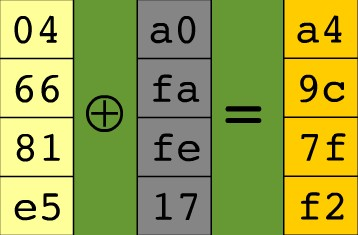
\includegraphics[width=0.3\textwidth]{img/S009.jpg}
    \caption{AddRoundKey}
\end{figure}

\FloatBarrier{}
\subsection{Генерация раундовых ключей}
\begin{figure}[h]
    \centering
    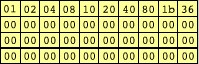
\includegraphics{img/S010.jpg}
    \caption{Rcon}
\end{figure}

\begin{enumerate}
    \item К столбцу матрицы ключа применяется побайтовый сдвиг на 1, SubBytes, его xor сложение с первым столбцом матрицы ключа и Rcon
    \begin{figure}[h]
        \centering
        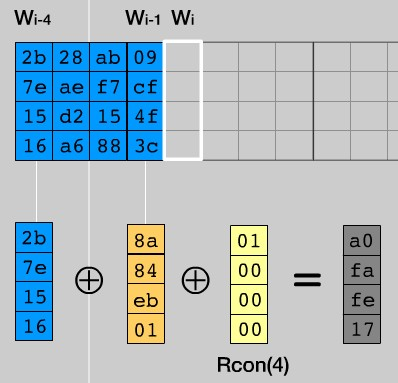
\includegraphics[width=0.5\textwidth]{img/S011.jpg}
        \caption{Первый столбец первого раундового ключа}
    \end{figure}
    \item Оставшиеся слова вычисляются xor'ом предыдущего слова со словом 4 позиции назад
    \begin{figure}[h]
        \centering
        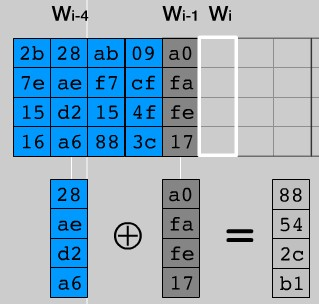
\includegraphics[width=0.5\textwidth]{img/S012.jpg}
        \caption{Второй столбец первого раундового ключа}
    \end{figure}
    \FloatBarrier{}
    \item Второй ключ вычисляется аналогичным образом по первому и т.д.
\end{enumerate}

\section*{Выводы}

\end{document}
